\section{Correlation}\label{sec:results}
Using Ca II H\&K emission data from \citet{Boudreaux2022} and
\citet{Perdelwitz2021} \citep[quantified using the $R'_{HK}$
metric][]{Middelkoop1982, Rutten1984} we investigate the correlation between
the Jao Gap magnitude and stellar magnetic activity. We are more statistically
limited here than past authors have been due to the requirement for high
resolution spectroscopic data when measuring Calcium emission; however, this is
balanced by an apparent stronger correlation between Calcium emission and the
Jao Gap when compared to H$\alpha$ emission. 

The merged dataset is presented in Figure \ref{fig:mergedData}. There is a
visual discontinuity just below the Jao Gap magnitude; however, this
manifests as an increase in the spread of the emission measurements rather than
a change in the mean value. In order to quantify the significance of this
discontinuity we measure the false alarm probability of the change in standard
deviation.

\begin{figure}
  \centering
  \includegraphics[width=0.45\textwidth]{Combined.pdf}
  \caption{Merged Dataset from \citet{Perdelwitz2021, Boudreaux2022}. Note the
  increase in the spread of $R'_{HK}$ around the Jao Gap Magnitude.}
  \label{fig:mergedData}
\end{figure}

First we split the merged dataset into bins with a width of 0.5 mag. In each bin we
measure the standard deviation about the mean of the data. The results of this
are shown in Figure \ref{fig:deviation}. In order to measure the false alarm
probability of this discontinuity we first resample the merged calcium
emission data based on the associated uncertainties for each datum as
presented in their respective publications. Then, for each of these ``resample
trials'' we measure the probability that a change in the standard deviation of
the size seen would happen purely due to noise. Results of this test are show in
in Figure \ref{fig:dist}. 

\begin{figure}
  \centering
  \includegraphics[width=0.45\textwidth]{Deviation.pdf}
  \caption{Standard deviation of Calcium emission data within each bin. Note
  the discontinuity near the Jao Gap Magnitude.}
  \label{fig:deviation}
\end{figure}

\begin{figure}
  \centering
  \includegraphics[width=0.45\textwidth]{fpDist.pdf}
  \caption{Probability distribution of the false alarm probability for the
  discontinuity seen in Figure \ref{fig:deviation}. The mean of this
  distribution is $0.341\%\pm^{0.08}_{0.08}$.}
  \label{fig:dist}
\end{figure}

This rapid increase star-to-star variability would only arise due purely to
noise $0.3\pm0.08$ percent of the time and is therefore likely either a true
effect or an alias of some sample bias.

If the observed increase in variability is not due to a sample bias and rather
is a physically driven effect then there is an obvious similarity between these
findings and those of \citet{Jao2023}. Specifically we find a increase in
variability just below the magnitude of the Gap. Moreover, this variability
increase is primarily driven by an increase in the number of low activity stars
(as opposed to an increase in the number of high activity stars). We can
further investigate the observed change in variability for only low activity
stars by filtering out those stars at or above the saturated threshold for
magnetic activity. \citet{Boudreaux2022} identify $\log(R'_{HK}) = -4.436$ as
the saturation threshold. We adopt this value and filter out all stars where
$\log(R'_{HK}) \geq -4.436$. Applying the same analysis to this reduced dataset
as was done to the full dataset we still find a discontinuity at the same
location (Figure \ref{fig:reduced}). This discontinuity is of a smaller
magnitude and consequently is more likely to be due purely to noise, with a
$7\pm0.2$ percent false alarm probability. This false alarm probability is
however only concerned with the first point after the jump in variability. If
we consider the false alarm probability of the entire high variability region
then the probability that the high variability region is due purely to noise
drops to $1.4\pm0.04$ percent.

\begin{figure}
  \centering
  \includegraphics[width=0.45\textwidth]{ReducedDeviation.pdf}
  \caption{Spread in the magnetic activity metric for the merged sample with
  any stars $\log(R'_{HK}) > -4.436$ filtered out.}
  \label{fig:reduced}
\end{figure}

We observe a strong, likely statistically significant, discontinuity in the
star-to-star variability of Ca II H\&K emission just below the magnitude
of the Jao Gap. However, modeling is required to determine if this discontinuity
may be due to the same underlying physics.

While the observed increase in variability seen here does not seem to be
coincident with the Jao Gap --- instead appearing to be approximately 0.5 mag
fainter, in agreement with what is observed in \citet{Jao2023} --- a number of
complicating factors prevent us from falsifying that the these two features are
not coincident. \citeauthor{Jao2023} find, similar to the results presented
here, that the paucity of $H\alpha$ emission originates just below the Gap.
Moreover, we use a 0.5 magnitude bin size when measuring the star-to-star
variability which injects error into the positioning of any feature in
magnitude space. We can quantify the degree of uncertainty the magnitude bin
choice injects by conducting Monte Carlo trials where bins are randomly shifted
redder or bluer. We conduct 10,000 trials where each trial involves sampling a
random shift to the bin start location from a normal distribution with a
standard deviation of 1 magnitude. For each trial we identify the discontinuity
location as the maximum value of the gradient of the standard deviation (this
is the derivative of the data in Figures \ref{fig:deviation} \&
\ref{fig:reduced}). Some trials result in the maximal value lying at the 0th
index of the magnitude array due to edge effects, these trials are rejected
(and account for 11\% of the trials). The uncertainty in the identified
magnitude of the discontinuity due to the selected start point of the magnitude
bins reveals a $1\sigma = \pm$0.32 magnitude uncertainty in the location of the
discontinuity (Figure \ref{fig:GapLocationMC}). Finally, all previous studies
of the M dwarf Gap \citep{Jao2018, Jao2021, Mansfield2021, Boudreaux2022,
Jao2023} demonstrate that the Gap has a color dependency, shifting to fainter
magnitudes as the population reddens and consequently an exact magnitude range
is ill-defined. Therefore we cannot falsify the model that the discontinuity in
star-to-star activity variability is coincident with the Jao Gap magnitude.

\begin{figure}
  \centering
  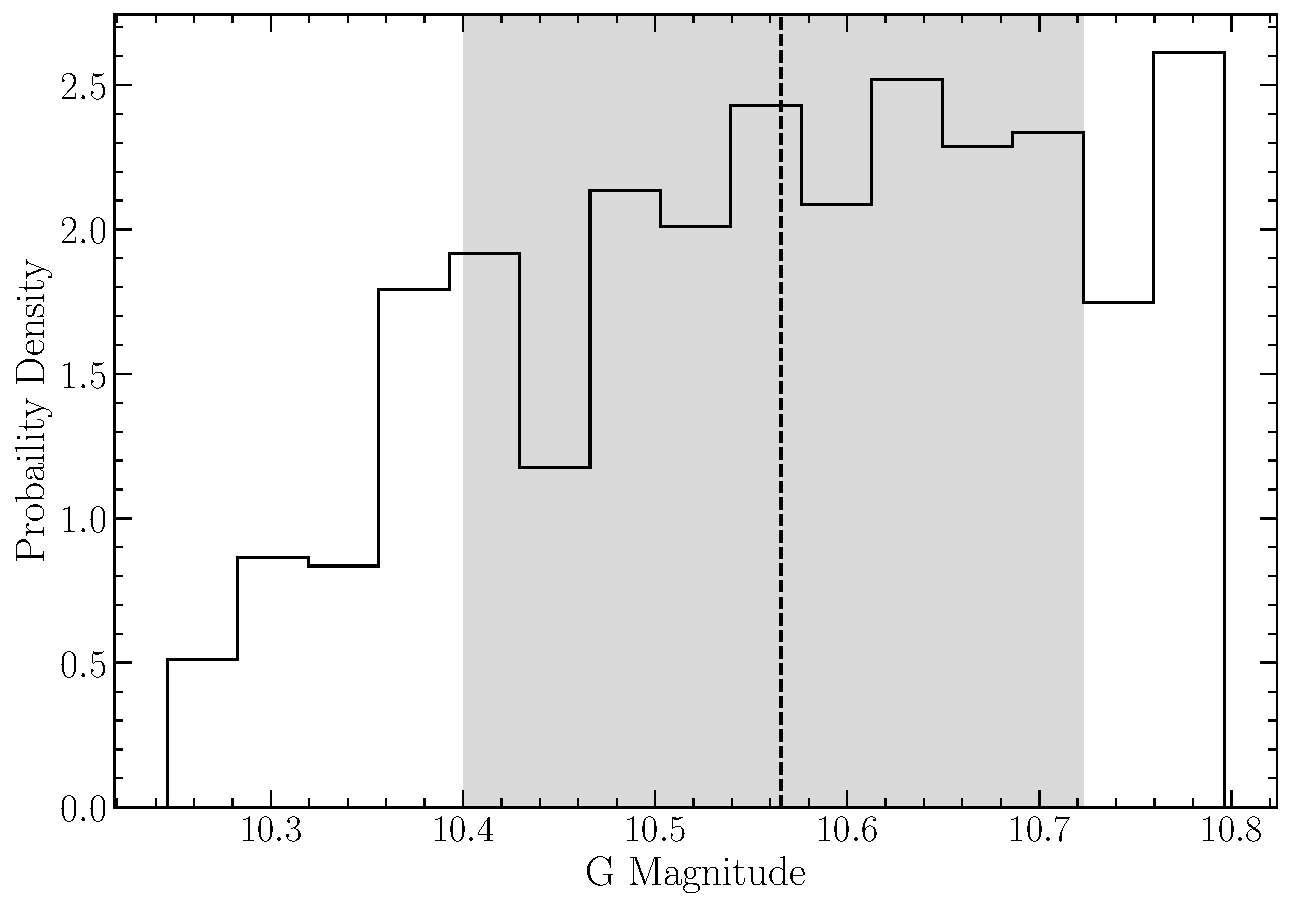
\includegraphics[width=0.45\textwidth]{GapLocationMC.pdf}
  \caption{Probability density distribution of discontinuity location as
  identified in the merged dataset. The dashed line represents the mean of the
  distribution while the shaded region runs from the 16th percentile to the
  84th percentile of the distribution. This distribution was built from 10,000
  independent samples where the discontinuity was identified as the highest
  value in the gradient of the standard deviation.}
  \label{fig:GapLocationMC}
\end{figure}

\subsection{Rotation}
It is well known that star's magnetic activity tend to be correlated with their
rotational velocity \citep{Vaughan1981, Newton2016, Astudillo-Defru2017,
Houdebine2017, Boudreaux2022}; therefore, we investigate whether there is a
similar correlation between Gap location and rotational period in our dataset.
All targets from \citet{Boudreaux2022} already have published rotational
periods; however, targets from \citet{Perdelwitz2021} do not necessarily have
published periods. Therefore, we derive photometric rotational periods for
these targets here. Given the inherent heterogeneity of M Dwarf stellar
surfaces \citep{Boisse2011, Robertson2020} we are able to determine the rotational period
of a star through the analysis of active regions. Various methodologies can be
employed for this purpose, including the examination of photometry and light
curves \citep[e.g.,][]{Newton2016}, and the observation of temporal changes in
the strength of chromospheric emission lines such as Ca II H \& K or H$\alpha$
\citep[e.g.,][]{2019A&A...623A..24F,2023MNRAS.518.3147K}. In this work, new rotational periods
are derived from TESS 2-minute cadence data\footnote{Some M Dwarfs lacking a
documented rotational period did not have sufficient TESS data to yield
fiducial rotational periods}.

Due to both the large frequency and amplitudes of M dwarf flaring rates the
photometric period can prove difficult to measure --- as frequency directly
correlates with periodicity. Thus, following the process described in
\citet{2023AJ....165..192G}, we utilize two methods in this paper to reduce the
effect of flares. One method uses \texttt{stella} a python package which
implements a series of pre-trained convolutional neural networks (CNNs) to
remove flare-shaped features in a light curve \citep{FeinsteinStella2020}. The
second method separates a star's photometry into 10 minute bins to account for
misshapen flares which \texttt{stella} is known to be biassed against detecting.

\texttt{stella}  employs a diverse library of models trained with varying
initial seeds \citep{FeinsteinFlare2020,FeinsteinStella2020}. The Convolutional
Neural Networks in \texttt{stella} are trained on labeled TESS 2-min for both
flares and non-flares. For the purposes of this paper, we use an ensemble of
100 models in \texttt{stella}'s library to optimize model performance
\citep[][for further detail]{FeinsteinFlare2020}. \texttt{stella} scores
flairs with a probability of between 0 to 1 --- where higher values indicate a
higher confidence that a feature is a flare. Here we adopt a score of 0.5 as
the cutoff threshold, all features with a score of 0.5 or greater are classed
as flares and removed \citep[e.g.][]{FeinsteinFlare2020}.

Furthermore, we also bin the data from a 2-min to 10-min cadence using the
python package \texttt{lightkurve}'s binning function
\citep{LightkurveCollaborationLightkurve2018,GeertBarentsenKeplerGO2020}. This
further reduces any flaring-contribution that might have been missed by
\texttt{stella}\footnote{This is relevant for flares that are misshapen at the
start or break in the dataset due to missing either the ingress or egress.}.
Subsequently, we filter photometry, only retaining data whos residuals are
less than 4 times the root-mean-square deviation.  

Gaussian processes for modeling the periods are based on
\citet{AngusInferring2018} for the subset of M Dwarfs with no fiducial periods.
The \texttt{starspot} \ package is adapted for light curve analysis
\citep{AngusRuthAngus2021, Angus2023}. Our Gaussian process kernel function
incorporates two stochastically-driven simple harmonic oscillators,
representing primary ($P_\textrm{rot}$) and secondary ($P_\textrm{rot}/2$)
rotation modes. First, we implement the Lomb-Scargle periodogram within
\texttt{starspot} to initially estimate the period. After which, we create a
maximum a posteriori (MAP) fit using \texttt{starspot} to generate a model for
stellar rotation. To obtain the posterior of the stellar rotation model, we use
Markov Chain Monte Carlo (MCMC) sampling using the \texttt{pymc3} package
\citep{SalvatierProbabilistic2016} within our adapted \texttt{starspot}
version. All rotational periods are presented in Table \ref{tab:dataset}. Our
final sample contains 187 stars with measured rotational periods. We derive new
rotational periods for 7 of these. 

\begin{deluxetable*}{cccccccc}
\tablehead{\colhead{ID} & \colhead{G Mag} & \colhead{V Mag} & \colhead{K Mag} & \colhead{R'$_{HK}$} & \colhead{R'$_{HK}$ err} & \colhead{Ro} & \colhead{prot}\\ \colhead{ } & \colhead{$\mathrm{mag}$} & \colhead{$\mathrm{mag}$} & \colhead{$\mathrm{mag}$} & \colhead{ } & \colhead{ } & \colhead{ } & \colhead{$\mathrm{d}$}}
\startdata
2MASS J00094508-4201396 & 12.140126 & 13.659000 & 8.223000 & -4.339205 & 0.001061 & 0.008610 & 0.859000 \\
2MASS J00310412-7201061 & 12.300688 & 13.648000 & 8.445000 & -5.387898 & 0.003143 & 0.928044 & 80.969000 \\
2MASS J01040695-6522272 & 12.447152 & 13.950000 & 8.532000 & -4.488843 & 0.001365 & 0.006320 & 0.624000 \\
2MASS J02004725-1021209 & 12.778251 & 14.113000 & 9.092000 & -4.790731 & 0.001247 & 0.188281 & 14.793000 \\
2MASS J02014384-1017295 & 13.026334 & 14.477000 & 9.189000 & -4.540044 & 0.001256 & 0.034402 & 3.152000 \\
2MASS J02125458+0000167 & 12.096099 & 13.580000 & 8.168000 & -4.634546 & 0.000999 & 0.048089 & 4.732000 \\
2MASS J02411510-0432177 & 12.250948 & 13.790000 & 8.246000 & -4.427184 & 0.001131 & 0.003768 & 0.400000 \\
2MASS J03100305-2341308 & 12.230226 & 13.500000 & 8.567000 & -4.233516 & 0.001114 & 0.027889 & 2.083000 \\
2MASS J03205178-6351524 & 12.086746 & 13.433000 & 8.195000 & -5.628891 & 0.004073 & 1.029200 & 91.622000 \\
2MASS J05015746-0656459 & 10.649305 & 12.196000 & 6.736000 & -5.004865 & 0.002015 & 0.874869 & 88.500000
\enddata

\caption{First 10 rows of the dataset used in this work. This data is avalible as a machine readable supliment to this article.}
\label{tab:dataset}

\end{deluxetable*}


One might expect a decrease in mean rotational period around the magnitude of
the Gap, due to the slight decrease in magnetic activity. However, there is no
statistically significant correlation between rotational period and G
magnitude which we can detect given our sample size (Figure
\ref{fig:rotationalSignifigance}). Rotational period is however, not the ideal
parametrization to use, as magnetic activity is more directly related to the
Rossby number ($Ro$). Using the empirical calibration presented in
\citet{Wright2018} (Equation \ref{eqn:tauc}) we find the mixing timescale for
each star such that the Rossby Number is defined as $Ro = P_{rot}/\tau_{c}$.

\begin{equation}\label{eqn:tauc}
  \tau_{c} = 0.64 + 0.25 * (V-K)
\end{equation}

When we compare Rossby number to G magnitude (Figure \ref{fig:rossby}) we find
that there may be a slight paucity of rotation coincident with the decrease in
spread of the activity metric. We quantify the statistical significance of this
drop by building a Gaussian kernel density estimator (kde) based on the data
outside of this range, and then resampling that kde 10000 times for each data
point in the theorized paucity range. The false alarm probability that that drop
is due to noise is then the product of the fraction of samples which are less
than or equal to the value of each data point. We find that there is a 0.022
percent probability that this dip is due purely to noise.


\begin{figure}
  \centering
  \includegraphics[width=0.45\textwidth]{RotationSignifigance.pdf}
  \caption{Rotational Periods against G magnitude for all stars with rotational
  periods (top). Standard deviation of rotational period within magnitude bin (bottom).}
  \label{fig:rotationalSignifigance}
\end{figure}

\begin{figure}
  \centering
  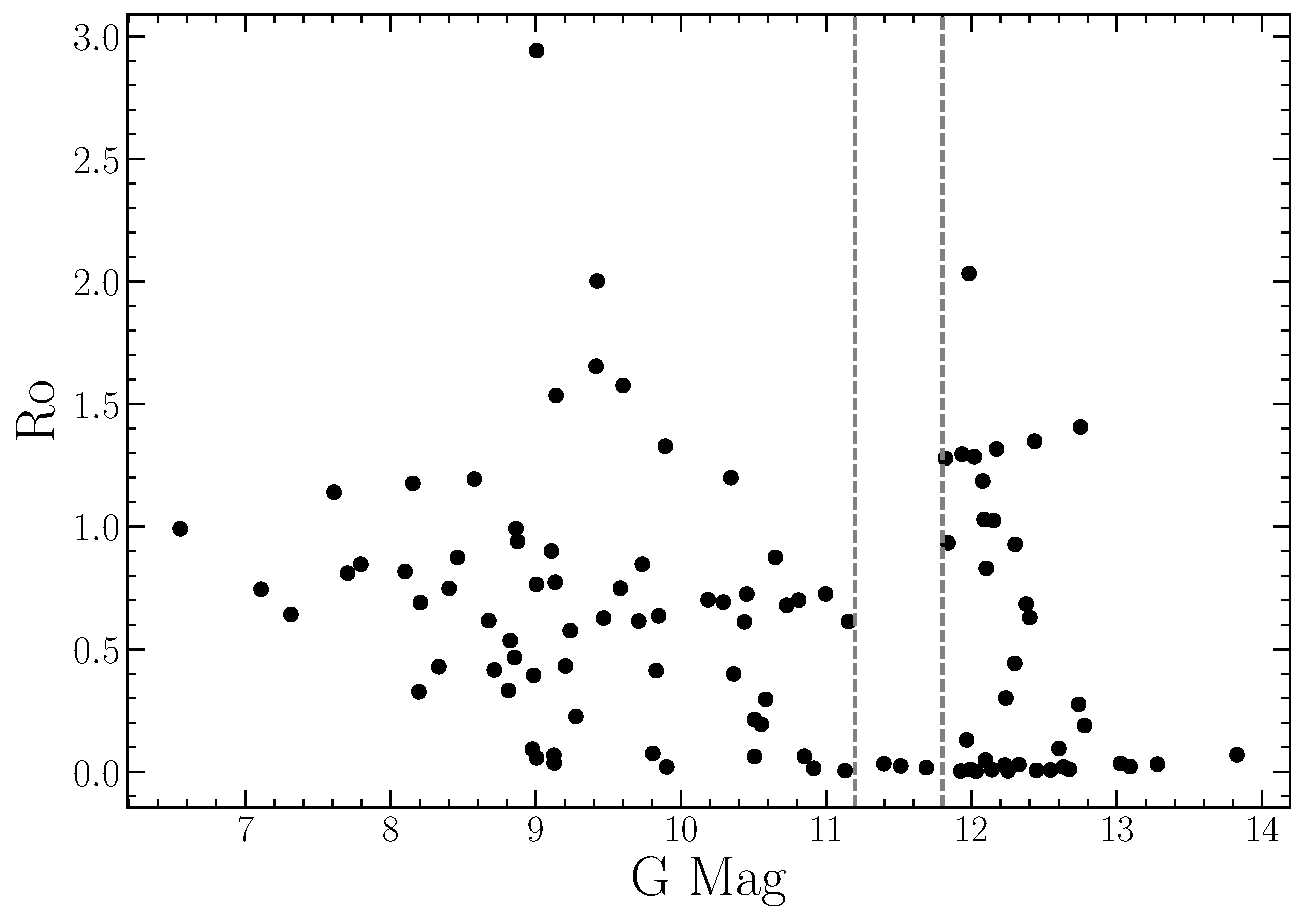
\includegraphics[width=0.45\textwidth]{Rossby.pdf}
  \caption{Rossby number vs. G magnitude for all stars with rotational periods
  and V-K colors on Simbad. Dashed lines represent the hypothesized region of decreased rotation.}
  \label{fig:rossby}
\end{figure}


\subsection{Limitations}
There are two primary limitation of our dataset. First, we only have 264 star
in our dataset (with measured $R'_{HK}$, 187 with rotational periods) limiting
the statistical power of our analysis. This is primarily due to the relative
difficulty of obtaining Ca II H\&K measurements compared to obtaining $H\alpha$
measurements. Reliable measurements require both high spectral resolutions (R
$\sim$ 16000) and a comparatively blue wavelength range \footnote{wrt. to what
many spectrographs cover. There is no unified resource listing currently
commissioned spectrographs; however, it is somewhat hard to source glass which
transmits well at H\&K wavelengths limiting the lower wavelength of most
spectrographs.}.

Additionally, the sample we do have does not extend to as low mass as would be
ideal. This presents a degeneracy between two potential causes for the observed
increased star-to-star variability. One option, as presented above and
elaborated on in the following section, is that this is due to kissing
instabilities. However, another possibility is that this increased variability
is intrinsic to the magnetic fields of fully convective stars. This alternate
option may be further supported by the shape of the magnetic activity spread vs.
G magnitude relation. Convective kissing instabilities are not expected to
continue to much lower masses than the fully convective transition mass. The
fact that the increase in variance which we observe continues to much fainter
magnitudes would therefore be somewhat surprising in a purely convective kissing
instability driven framework (though the degeneracy between potentially
physically driven increase in variance and increase in variance due to the
noise-magnitude relation complicates attempts to constrain this.) There is
limited discussion in the literature of overall magnetic field strength
spanning the fully convective transition mass; however, \citet{Shulyak2019}
present estimated magnetic field strengths for 47 M dwarfs, spanning a larger
area around the convective transition region and their dataset does not
indicate a inherently increased variability for fully convective stars.
